\newpage
\def\thoigian{90}%--Thời gian
\de{Đề số 3}{Chương III. Hàm số bậc hai và đồ thị}



\begin{center}
	\textbf{PHẦN 1 - CÂU TRẮC NGHIỆM BỐN PHƯƠNG ÁN}
\end{center}
\Opensolutionfile{ans}[ans/ans-TN-ONTAPCHUONG-DE3]
\setcounter{ex}{0}
%Câu 1
\begin{ex}%[0D3N1-1]%[Dự án D - đợt 4 NH24-25- Lê Minh Thiện Anh]
	Biểu thức nào sau đây \textbf{không} là hàm số theo biến $x$?
		\choice
		{$y=\sqrt{x^2-1}$}
		{\True $y^4=x^3$}
		{$y=5x^2-3x+4$}
		{$y=x$}
	\loigiai{
		Vì với $x=1$ thì $y=\pm 1$ nên biểu thức $y^4=x^3$ không là hàm số theo biến $x$.
	}
\end{ex}

%Câu 2
\begin{ex}%[0D3N1-1]%[Dự án D - đợt 4 NH24-25- Lê Minh Thiện Anh]
	Hình vẽ nào dưới đây biểu diễn đồ thị của một hàm số?
		\def\dotEX{} 
		\choice
			{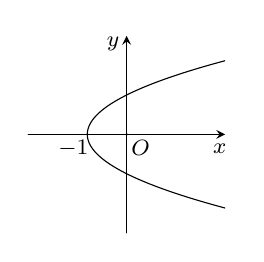
\begin{tikzpicture}[>=stealth,line join=round, line cap=round, scale=0.5,font=\footnotesize]
				\def \xmin{-2.5}\def \xmax{2.5}\def \ymin{-2.5}\def \ymax{2.5} 	
				\draw[->] (\xmin,0)--(\xmax,0) node[shift=(-110:0.2)] {$x$};
				\draw[->] (0,\ymin)--(0,\ymax) node[shift=(-150:0.2)] {$y$}; 
				\fill (0,0) circle(1pt) node[shift=(-45:0.25)]{$O$} (-1,0) circle(1pt) node[shift=(-135:0.25)]{$-1$}; 
				\clip (\xmin,\ymin) rectangle (\xmax,\ymax); 
				\draw[smooth,samples=100,domain=\xmin:\xmax] plot({(\x)^2-1},\x); 
			\end{tikzpicture}
			}
			{\begin{tikzpicture}[>=stealth,line join=round, line cap=round, scale=0.5,font=\footnotesize]
				\def \xmin{-1.5}\def \xmax{3.5}\def \ymin{-2.5}\def \ymax{2.5} 	
				\draw[->] (\xmin,0)--(\xmax,0) node[shift=(-110:0.2)] {$x$};
				\draw[->] (0,\ymin)--(0,\ymax) node[shift=(-30:0.2)] {$y$}; 
				\fill (0,0) circle(1pt) node[shift=(-135:0.25)]{$O$} (2,0) circle(1pt) node[shift=(-135:0.25)]{$2$}; 
				\clip (\xmin,\ymin) rectangle (\xmax,\ymax); 
				\draw[smooth,samples=100,domain=\ymin:\ymax] plot(2,\x); 
			\end{tikzpicture}
			}
			{\True 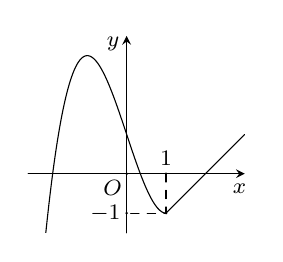
\begin{tikzpicture}[>=stealth,line join=round, line cap=round, scale=0.5,font=\footnotesize]
				\def \xmin{-2.5}\def \xmax{3}\def \ymin{-1.5}\def \ymax{3.5} 	
				\draw[->] (\xmin,0)--(\xmax,0) node[shift=(-110:0.2)] {$x$};
				\draw[->] (0,\ymin)--(0,\ymax) node[shift=(-150:0.2)] {$y$}; 
				\fill (0,0) circle(1pt) node[shift=(-135:0.25)]{$O$} 
					(1,0) circle(1pt) node[shift=(90:0.2)]{$1$}
					(0,-1) circle(1pt) node[shift=(180:0.27)]{$-1$}
					(1,-1) circle(1pt); 
				\clip (\xmin,\ymin) rectangle (\xmax,\ymax); 
				\draw[smooth,samples=100,domain=\xmin:1] plot(\x,{(\x)^3-3*(\x)+1}); 
				\draw[smooth,samples=100,domain=1:\xmax] plot(\x,{(\x)-2});
				\draw[dashed] (1,0) --(1,-1)--(0,-1);
			\end{tikzpicture}
			}
			{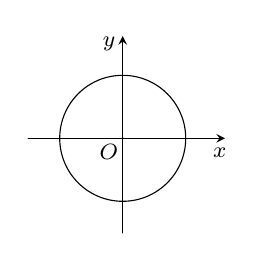
\begin{tikzpicture}[>=stealth,line join=round,font=\footnotesize, line cap=round, scale=0.4]
				\def \xmin{-3}\def \xmax{3.25}\def \ymin{-3}\def \ymax{3.25} 	
				\draw[->] (\xmin,0)--(\xmax,0) node[shift=(-110:0.2)] {$x$};
				\draw[->] (0,\ymin)--(0,\ymax) node[shift=(-150:0.2)] {$y$}; 
				\fill (0,0) circle(1pt) node[shift=(-135:0.25)]{$O$}; 
				\draw (0,0) circle (2) ;
			\end{tikzpicture}
			}
		\loigiai{
			Hình vẽ  biễu diễn đồ thị của một hàm số là 
			\begin{center}
	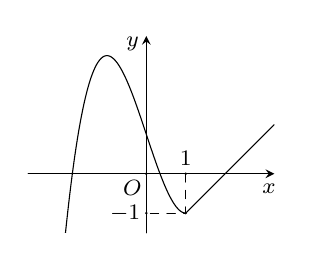
\begin{tikzpicture}[>=stealth,line join=round, line cap=round, scale=0.5,font=\footnotesize]
				\def \xmin{-3}\def \xmax{3.25}\def \ymin{-1.5}\def \ymax{3.5} 	
				\draw[->] (\xmin,0)--(\xmax,0) node[shift=(-110:0.2)] {$x$};
				\draw[->] (0,\ymin)--(0,\ymax) node[shift=(-150:0.2)] {$y$}; 
				\fill (0,0) circle(1pt) node[shift=(-135:0.25)]{$O$} 
					(1,0) circle(1pt) node[shift=(90:0.2)]{$1$}
					(0,-1) circle(1pt) node[shift=(180:0.27)]{$-1$}
					(1,-1) circle(1pt); 
				\clip (\xmin,\ymin) rectangle (\xmax,\ymax); 
				\draw[smooth,samples=100,domain=\xmin:1] plot(\x,{(\x)^3-3*(\x)+1}); 
				\draw[smooth,samples=100,domain=1:\xmax] plot(\x,{(\x)-2});
				\draw[dashed] (1,0) --(1,-1)--(0,-1);
			\end{tikzpicture}
			\end{center}
		Các hình vẽ còn lại  không thỏa mãn định nghĩa hàm số, vì mỗi giá trị $x$ có thể có tương ứng nhiều hơn $1$ giá trị $y$.
		}
\end{ex}
	
%Câu 3
\begin{ex}%[0D3N1-2]%[Dự án D - đợt 4 NH24-25- Lê Minh Thiện Anh]
	Tập xác định của hàm số $y=\dfrac{x-2}{x-3}$ là
	\choice
	{ $\{2\}$}
	{ $ \mathbb{R} \setminus\{3\}$}
	{ $\mathbb{R}\setminus\{2\}$}
	{ $\{3\}$}
	\loigiai{
		Hàm số xác định khi và chỉ khi $x-3\neq 0\Leftrightarrow x\neq 3$.\\
		Vậy $\mathscr{D}=\mathbb{R}\setminus \{3\}$.
	}
\end{ex}

%Câu 4
\begin{ex}%[0D3H1-3]%[Dự án D - đợt 4 NH24-25- Lê Minh Thiện Anh]
	Cho hàm số $y=ax^2$ $(a \neq 0)$ có đồ thị như hình bên dưới
	\begin{center}
	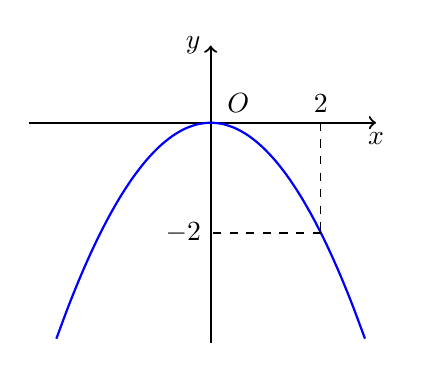
\begin{tikzpicture}[x=0.7 cm,y=0.7 cm]
		\def\f(#1){- 0.5*(#1)^2}
		% Tiến hành vẽ hai trục tọa độ
		\draw[->, color=black, thick] (-3.3,0) -- (3,0) node[below] {$x$}; %Vẽ trục Ox từ tọa độ () đến tạo độ (), màu đen và độ dày là thick và có đánh dấu mũi tên ->
		\draw[->,color=black,thick] (0,-4) -- (0,1.4) node[left]{$y$}; %vẽ trục oy
		%Vẽ đồ thị
		\draw[smooth, blue,thick] plot[domain=-2.8:2.8](\x,{\f(\x)});
		%Ve cac diem
		\draw (0.5,0)  node[above]{$O$};
		\draw (2,0)  node[above]{$2$};
		\draw (0,-2)  node[left]{$-2$};
		\draw[dashed] (2,0)--(2,-2);
		\draw[dashed] (2,-2)--(0,-2);
	\end{tikzpicture}
	\end{center}
	Hàm số đã cho có tập giá trị là
		\choice
		{$(-\infty;0)$}
		{$(-\infty;+\infty)$}
		{\True $\left( -\infty; 0 \right]$}
		{$(-2;2)$}
		\loigiai{Dựa vào đồ thị, ta xác định được tập giá trị của hàm số là  $\left( -\infty; 0 \right]$.}
\end{ex}

%Câu 5
\begin{ex}%[0D3H1-3]%[Dự án D - đợt 2 NH24-25- Lê Minh Thiện Anh]
	Cho hàm số $f(x)=\heva{& -2x+1 & \text{ khi } x\le 0 \\
			& 2x^2-x+1 & \text{ khi } x > 0}$. Giá trị của $f(1)+f(-1)$ bằng
	\choice
	{$3$}
	{$2$}
	{\True $5$}
	{$0$}
	\loigiai{
		Ta có $f(-1)=-2\cdot (-1)+1=3$ và $f(1)=2-1+1=2$.\\
		Vậy $f(1)+f(-1)= 5$.
	}
\end{ex}

%Câu 6
\begin{ex}%[0D3H1-2]%[Dự án D - đợt 4 NH24-25- Lê Minh Thiện Anh]
	Tập xác định $\mathscr{D}$ của hàm số $y=f(x)= \dfrac{x+3}{\sqrt{x-2}}$ là
	\choice
	{\True $\mathscr{D}=\left( 2;+\infty \right)$}
	{ $\mathscr{D}=\left( -3;+\infty \right)$}
	{ $\mathscr{D}=\left[ 2;+\infty \right)$}
	{ $\mathscr{D}=\left[ -3;+\infty \right)$}
	\loigiai{
		Điều kiện $x-2>0 \Leftrightarrow x>2$.\\
		Vậy tập xác định là $\mathscr{D}=(2;+\infty)$.}
\end{ex}

%Câu 7
\begin{ex}%[0D3N2-1]%[Dự án D - đợt 4 NH24-25- Lê Minh Thiện Anh]
	Hoành độ đỉnh của parabol $(P)\colon y=x^2-6x+1$ là
	\choice
	{\True $x=3$}
	{$x=6$}
	{$x=-3$}
	{$y=3$}
	\loigiai{
		Hoành độ đỉnh $x=-\dfrac{b}{2a}=-\dfrac{-6}{2\cdot1}=3$.
	}
\end{ex}

%Câu 8
\begin{ex}%[0D3H2-2]%[Dự án D - đợt 4 NH24-25- Lê Minh Thiện Anh]
	Hàm số $y=2x^2-4x-5$ đồng biến trên khoảng nào dưới đây?
	\choice
	{$(-\infty;-1)$}
	{$(-1;+\infty)$}
	{\True $(1;+\infty)$}
	{$(-\infty;1)$}
	\loigiai{
		Ta có $a=2>0$ và $-\dfrac{b}{2a}=1$ nên hàm số $y=2x^2-4x-5$ đồng biến trên khoảng $(1;+\infty)$.
	}
\end{ex}

%Câu 9
\begin{ex}%[0D3N2-1]%[Dự án D - đợt 4 NH24-25- Lê Minh Thiện Anh]
	Hàm số nào sau đây là hàm số bậc hai?
	\choice
	{\True $y=-3 x^{2}+2 x+5$}
	{$y=\dfrac{1}{2 x^{2}+2 x+1}$}
	{$y=4 x+3$}
	{$y=5 x-1$}
	\loigiai{
		Hàm số $y=-3 x^{2}+2 x+5$ là hàm số bậc hai.
	}
\end{ex}

%Câu 10
\begin{ex}%[0D3N2-1]%[Dự án D - đợt 4 NH24-25- Lê Minh Thiện Anh]
	Cho hàm số bậc hai $y=a x^2+b x+c$, $(a \neq 0)$ có đồ thị $(P)$, đỉnh của $(P)$ được xác định bởi công thức nào?
	\choice
	{ $I\left(\dfrac{b}{2 a} ; \dfrac{\Delta}{4 a}\right)$}
	{ $I\left(-\dfrac{b}{a} ;-\dfrac{\Delta}{4 a}\right)$}
	{\True  $I\left(-\dfrac{b}{2 a} ;-\dfrac{\Delta}{4 a}\right)$}
	{ $I\left(-\dfrac{b}{2 a} ; \dfrac{\Delta}{4 a}\right)$}
	\loigiai{
		Đỉnh của $(P)$ là $I\left(-\dfrac{b}{2 a} ;-\dfrac{\Delta}{4 a}\right)$.
}
\end{ex}

%Câu 11
\begin{ex}%[0D3H2-2]%[Dự án D - đợt 4 NH24-25- Lê Minh Thiện Anh]
	\immini{Đồ thị trong hình vẽ là của hàm số nào?
	\choice
	{$y=x^2+2x-1$}
	{$y=x^2+2x-2$}
	{$y=2x^2-4x-2$}
	{\True $y=x^2-2x-1$}
	}
	{
	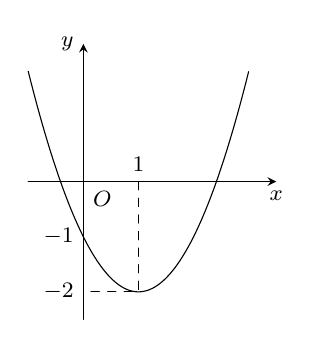
\begin{tikzpicture}[scale=0.7, font=\footnotesize, line join=round, line cap=round, >=stealth]
	\draw[->](-1,0)--(3.5,0)node[below]{$x$};
	\draw[->](0,-2.5)--(0,2.5)node[left]{$y$};
	\draw[smooth, samples=100, domain=-1:3]plot(\x,{(\x)^2-2*(\x)-1});
	\draw[dashed]
	(1,0)--(1,-2)--(0,-2)
	;
	\path
	(0,0)node[below right]{$O$}
	(1,0)node[above]{$1$}
	(0,-1)node[left]{$-1$}
	(0,-2)node[left]{$-2$}
	;
	\end{tikzpicture}
	}
	\loigiai{
		Vì các đáp án là hàm số bậc hai nên ta giả sử hàm số cần tìm là $y=ax^2+bx+c$. \\
		Từ hình vẽ, ta thấy đồ thị hàm số cắt trục tung $Oy$ tại điểm có tung độ $y=-1$ và tọa độ đỉnh $(1;-2)$.\\
		Suy ra $\heva{ & c=-1 \\ & -\dfrac{b}{2a}=1 \\ & a+b+c=-2} \Leftrightarrow \heva{ & c=-1 \\ & 2a+b=0 \\ & a+b+c=-2} \Leftrightarrow \heva{ & a=1 \\ & b=-2 \\ & c=-1.}$ \\
		Vậy hàm số cần tìm là $y=x^2-2x-1$.
		}
\end{ex}

%Câu 12
\begin{ex}%[0D3H2-2]%[Dự án D - đợt 4 NH24-25- Lê Minh Thiện Anh]
	\immini[thm]{Cho hàm số $y=ax^2+bx+c$ $(a$, $b$, $c \in \mathbb{R})$ có đồ thị như hình vẽ bên. Khẳng định nào sau đây là đúng?
			\choice[2]
			{$a>0$; $b<0$; $c>0$}
			{$a<0$; $b<0$; $c>0$}
			{\True $a<0$; $b>0$; $c>0$}
			{$a>0$; $b>0$; $c>0$}
		}{	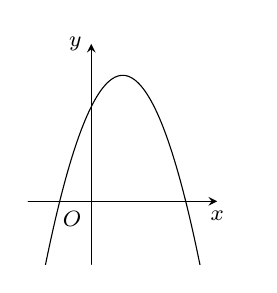
\begin{tikzpicture}[scale=.4, font=\footnotesize, line join=round, line cap=round, >=stealth]
				\def\a{-1} % Hệ số a phải khác 0
				\def\b{2}
				\def\c{3}
				\draw[->] (-2,0) -- (4,0) node[below] {$x$};
				\draw[->] (0,-2) -- (0,5) node[left] {$y$};
				\fill (0,0) circle node[below left]{$O$};
				\pgfmathsetmacro\xdinh{-(\b)/2*(\a)}			\pgfmathsetmacro\ydinh{(4*(\a)*(\c)-(\b)^2)/(4*(\a))}
				\clip (-2,-2)rectangle(5,5);	\draw[samples=150,smooth,domain=-5:5] plot(\x,{\a*(\x)^2+(\b)*\x+(\c)});
		\end{tikzpicture}}
		\loigiai{
			Dựa vào đồ thị bên, ta có
			\begin{itemize}
				\item Đồ thị có bề lõm hướng xuống nên $a<0$.
				\item Đồ thị cắt trục tung tại điểm $(0;c)$ có tung độ dương nên $c>0$.
				\item Đồ thị có hoành độ đỉnh dương nên $-\dfrac{b}{2a}>0 \Leftrightarrow \dfrac{b}{a}<0 $ và do $a<0$ nên $b>0$.
			\end{itemize}
		}
\end{ex}
\Closesolutionfile{ans}
%\begin{center}
%	\textbf{ĐÁP ÁN}
%	\inputansbox{10}{ans/ans}	
%\end{center}



\begin{center}
	\textbf{PHẦN 2 - CÂU TRẮC NGHIỆM ĐÚNG SAI}
\end{center}
\setcounter{ex}{0}
\Opensolutionfile{ans}[ans/answer-DS-ONTAPCHUONG-DE3]
\begin{ex}%[0D3H1-3]%[Dự án D - đợt 4 NH24-25- Lê Minh Thiện Anh]
	Cho hàm số $f(x)=\heva{&x^2+3x+1 &\text{khi} \ x \leq 1\\&-x+6 &\text{khi} \ x>1.}$
	\choiceTF
	{\True Hàm số có tập xác định $\mathscr{D}=\mathbb{R}$}
	{$f(-1)=3$}
	{Hàm số đồng biến trên khoảng $(1;+\infty)$}
	{\True Gọi $S$ là tập các giá trị của $x$ để $f(x)=1$, tổng các phần tử của $S$ là $2$}
	\loigiai{
		\begin{itemchoice}
			\itemch Tập xác định của hàm số $\mathscr{D}=(-\infty;1]\cup (1;+\infty) =\mathbb{R}$.
			\itemch Vì $-1<1$ nên $f(-1)=(-1)^2+3\cdot (-1)+1=-1$.	
			\itemch Với $x>1$, ta có $f(x)=-x+6$ nên hàm số nghịch biến trên khoảng $(1;+\infty)$.
			\itemch 
			Với $x\leq 1$, ta có $f(x)=1 \Leftrightarrow x^2+3x+1=1 \Leftrightarrow \hoac{& x=0 \text{ (thỏa mãn)}\\& x=-3 \text{ (thỏa mãn)}.}$\\
			Với $x>1$, ta có $f(x)=1 \Leftrightarrow -x+6=1 \Leftrightarrow x=5 \text{ (thỏa mãn)}$.\\
			Vậy $S=\{-3;0;5\}$ và tổng các phần tử của $S$ bằng $2$.
			\end{itemchoice}
		}
\end{ex}

\begin{ex}%[0D3V2-4]%[Dự án D - đợt 4 NH24-25- Lê Minh Thiện Anh]
	Cho hàm số $y=-x^2+2mx+1$ có đồ thị $(P)$. Xét tính đúng sai của các mệnh đề sau.
	\choiceTF
	{Hàm số đã cho là hàm số bậc hai khi và chỉ khi $m\ne 0$}
	{\True Với $m=-2$ thì parabol $(P)$ có đỉnh là $I(-2;5)$}
	{Hàm số đồng biến trên $(-\infty;3)$ khi và chỉ khi $m=3$}
	{\True Có đúng một giá trị thực của tham số $m$ để đỉnh của parabol $(P)$ thuộc đường thẳng $y=2x$}
	\loigiai{
		\begin{itemchoice}
			\itemch Ta có $a=-1 \ne 0$ nên hàm số đã cho là hàm số bậc hai với mọi $m \in \mathbb{R}$.
			\itemch Khi $m=-2$ thì $y=-x^2-4x+1$ là parabol có đỉnh $I$
			$$\heva{&x_I =\dfrac{-b}{2a} =\dfrac{4}{2 \cdot (-1)}=-2\\& y_I = -(-2)^2-4 \cdot (-2)+1= 5} \Rightarrow I(-2;5).$$
			\itemch Ta có $a=-1<0$; $-\dfrac{b}{2a}=m$ nên hàm số đã cho đồng biến trên khoảng $(-\infty;m)$, nghịch biến trên khoảng $(m;+\infty)$.\\
			Do đó để hàm số đồng biến trên $(-\infty;3)$ thì $(-\infty;3) \subset (-\infty;m)$ hay $m \ge 3$.
			\itemch Ta có $x_I= \dfrac{-b}{2a} = m$ và $y_I = -m^2 +2m \cdot m +1 = m^2+1$. Do đó parabol $(P)$ có đỉnh $I\left(m;m^2+1\right)$.\\
			Điểm $I$ thuộc đường thẳng $y=2x$ nên
			$$ m^2+1 = 2m \Leftrightarrow m =1.$$
		\end{itemchoice}
	}
\end{ex}
\Closesolutionfile{ans}
%\inputansbox[2]{2}{ans/answer.tex}
\begin{center}
\textbf{PHẦN 3 - CÂU TRẮC NGHIỆM TRẢ LỜI NGẮN}
\end{center}
\setcounter{ex}{0}
\Opensolutionfile{ans}[ans-KQ-ONTAPCHUONG-DE3]
\begin{ex}%[0D3H1-3]%[Dự án D - đợt 4 NH24-25- Lê Minh Thiện Anh]
	Cho hàm số $f(x)=\dfrac{2x+m}{x+3}$ (với $m$ là tham số) có $f(-2)=-5$. Khi đó giá trị của $m$ là bao nhiêu?
	
	\shortans[oly]{$-1$} 
	\loigiai{
		Ta có $f(-2)=\dfrac{2\cdot(-2)+m}{-2+3}=-5 \Leftrightarrow \dfrac{-4+m}{1}=-5 \Leftrightarrow -4+m=-5 \Leftrightarrow m=-1$.
	}
\end{ex}

\begin{ex}%[0D3V1-7]%[Dự án D - đợt 4 NH24-25- Lê Minh Thiện Anh]
Bảng giá nước sinh hoạt ở địa phương A năm 2021 được cho như bảng dưới đây.
	\begin{center}
		\begin{tabular}{|>{\raggedright\arraybackslash}m{4.5cm}|>{\raggedleft\arraybackslash}m{4cm}|>{\raggedleft\arraybackslash}m{2.5cm}|>{\raggedleft\arraybackslash}m{2.5cm}|}
				\hline
				\begin{center}
					Mức sử dụng (m$^3$)
				\end{center} & \begin{center}
					Giá chưa thuế GTGT (VNĐ/m$^3$)
				\end{center} & \begin{center}
					Phí BVMT (VNĐ/m$^3$)
				\end{center} & \begin{center}
					Thuế GTGT (VNĐ/m$^3$)
				\end{center}\\
				\hline
				Từ trên $0$ m$^3$ đến $4$ m$^3$ & $5\,300$ & $530$ & $265$\\
				\hline
				Từ trên $4$ m$^3$ đến $6$ m$^3$& $10\,200$ & $1\,020$ & $510$\\
				\hline
				Trên $6$ m$^3$ & $11\,400$ & $1\,140$ & $570$\\
				\hline
		\end{tabular}
	\end{center}
	Biết rằng tháng 8 năm 2021 một hộ gia đình ở địa phương đó sử dụng hết $12$ m$^3$ nước sinh hoạt. Số tiền nước tháng 8/2021 gia đình đó phải nộp là bao nhiêu nghìn đồng (kết quả làm tròn đến nghìn đồng)?

	\shortans[oly]{127}
	\loigiai
	{Số tiền hộ gia đình phải nộp là
	\allowdisplaybreaks
	\begin{align*}
		T=&(5\,300+530+265)\cdot 4 + (10\,200+1020+510)\cdot 2 + (11\,400+1140+570)\cdot 6\\
		=& 126\,500 \text{ (đồng)}\\
		\approx &127 \text{ (nghìn đồng)}.
	\end{align*}}
\end{ex}

\begin{ex}%[0D3H2-1]%[Dự án D - đợt 4 NH24-25- Lê Minh Thiện Anh]
	Hàm số bậc hai $y=ax^2+bx+c$ có đồ thị là $(P)$ đi qua hai điểm $A(-1;6)$, $B(4;3)$ và có trục đối xứng là $x=2$. Tính giá trị của biểu thức $S=a-b+c$.
	
	\shortans[oly]{$6$}
	\loigiai{
		Vì trục đối xứng của $(P)$ là $x=2$ nên $-\dfrac{b}{2a}=2 \Leftrightarrow b=-4a$.\\
		Mặt khác hai điểm $A$, $B$ thuộc $(P)$ nên ta có
			\[\heva{&a-b+c=6\\&16a+4b+c=3} \Leftrightarrow \heva{&5a+c=6\\&c=3} \Leftrightarrow \heva{&a=\dfrac{3}{5}\\&c=3.}\]
		Suy ra $b=-4a=-\dfrac{12}{5}$.\\
		Vậy $S=a-b+c=\dfrac{3}{5}- \left(-\dfrac{12}{5}\right)+3=6$.
	}
\end{ex}

\begin{ex}%[0D3V2-6]%[Dự án D - đợt 4 NH24-25- Lê Minh Thiện Anh]
	\immini{Một cổng chào có hình parabol (tham khảo hình bên), biết khoảng cách giữa hai chân cổng bằng $20$\,m và điểm $M$ trên cổng có tọa độ $(2;6)$. Chiều cao $h$ (đơn vị m) của cổng (được làm tròn đến chữ số thập phân thứ nhất) bằng bao nhiêu?}
	{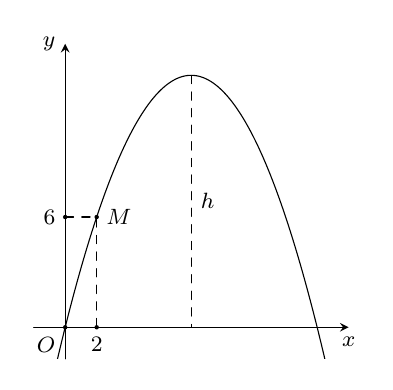
\begin{tikzpicture}[scale=0.8, font=\footnotesize, line join=round, line cap=round, >=stealth]
			\def\xmin{-0.5}\def\xmax{4.5}\def\ymin{-0.5}\def\ymax{4.5}
			\draw[->] (\xmin,0)--(\xmax,0) node[below] {$x$};
			\draw[->] (0,\ymin)--(0,\ymax) node[left] {$y$};
			\fill (0,0) circle (1pt) node [below left] {$O$} (0.5,1.75) circle (1pt) node [right] {$M$}
			(0,1.75) circle (1pt) node [left]{$6$}
			(0.5,0) circle (1pt) node [below]{$2$}
			;
			
			\clip (\xmin,\ymin) rectangle (\xmax,\ymax);
			\draw[smooth,samples=200,domain=\xmin:\xmax] plot (\x,{-1*((\x)^2)+4*\x});
			\draw [dashed] (2,4)--(2,2) node [right]{$h$}--(2,0);
			\draw [dashed] (0,1.75) --(0.5,1.75)--(0.5,0);
		\end{tikzpicture}
	}
	\shortans[oly]{$16{,}7$}
	\loigiai{
	\begin{center}
	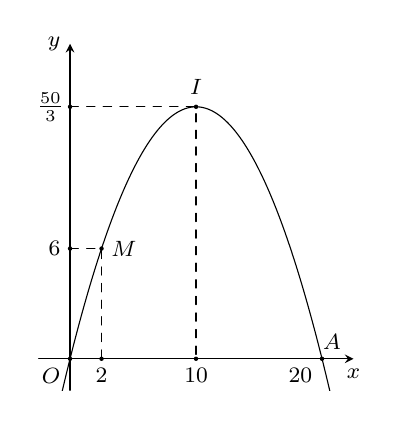
\begin{tikzpicture}[scale=0.8, font=\footnotesize, line join=round, line cap=round, >=stealth]
		\def\xmin{-0.5}\def\xmax{4.5}\def\ymin{-0.5}\def\ymax{5}
		\draw[->] (\xmin,0)--(\xmax,0) node[below] {$x$};
		\draw[->] (0,\ymin)--(0,\ymax) node[left] {$y$};
		\fill (0,0) circle (1pt) node [below left] {$O$} (0.5,1.75) circle (1pt) node [right] {$M$}
		(0,1.75) circle (1pt) node [left]{$6$}
		(0.5,0) circle (1pt) node [below]{$2$}
		(0,4) circle (1pt) node[shift=(180:0.25)]{$\frac{50}{3}$}
		(2,4) circle (1pt) node [shift=(90:0.25)]{$I$}
		(2,0) circle (1pt) node [below]{$10$} 
		(4,0) circle (1pt) node [below left]{$20$}
		;
		
		\clip (\xmin,\ymin) rectangle (\xmax,\ymax);
		\draw[smooth,samples=200,domain=\xmin:\xmax] plot (\x,{-1*((\x)^2)+4*\x});
		\draw (4,0) node [shift=(60:0.25)]{$A$};
		\draw [dashed] (0,1.75) --(0.5,1.75)--(0.5,0)
		(0,4)--(2,4)--(2,0)
		;
	\end{tikzpicture}
	\end{center}
	Giả sử parabol $(P)\colon y=ax^2+bx+c$ ($a \neq 0$).\\
	Do đồ thị hàm số cắt trục $Ox$ tại hai điểm $O(0; 0)$ và $A(20,0)$ nên ta có $\heva{&c=0\\&20^2a+20b=0.}$\\
	Lại có đồ thị hàm số đi qua $M(2;6)$ nên ta có $4a+2b=6$.\\
	Ta có hệ phương trình \[\heva{&400a+20b=0\\&4a+2b=6}\Leftrightarrow\heva{&a=-\dfrac{1}{6}\\&b=\dfrac{10}{3}.}\]
	Do đó $(P)\colon y=-\dfrac{1}{6}x^2+\dfrac{10}{3}x$.\\
	Parabol $(P)$ có đỉnh $I\left(10;\dfrac{50}{3}\right)$. Khi đó $h=y_I=\dfrac{50}{3}\approx 16{,}7$. 
		}
\end{ex}

\Closesolutionfile{ans}
\begin{center}
	\textbf{PHẦN 4 - TỰ LUẬN}
\end{center}
\setcounter{ex}{0}
%Câu 1...........................
\begin{ex}%[0D3V1-7]%[Dự án D - đợt 4 NH24-25- Lê Minh Thiện Anh]
	Một lớp muốn thuê một chiếc xe khách cho chuyến tham quan, có hai công ty được tiếp cận để tham khảo giá.\\
	Công ty A có giá khởi đầu là $3{,}75$ triệu đồng cộng thêm $5\,000$ đồng cho mỗi ki-lô-mét chạy xe.\\
	Công ty B có giá khởi đầu là $3$ triệu đồng cộng thêm $7\,500$ đồng cho mỗi ki-lô-mét chạy xe.\\
	Biết quãng đường chạy xe là $220$ km. Số tiền xe thấp nhất mà lớp phải trả khi lựa chọn xe của một trong hai công ty trên là bao nhiêu (tính theo đơn vị: triệu đồng)?
	\loigiai{
		Nếu lớp đó chọn công ty A thì số tiền xe phải trả là $$T_A=3{,}75+\dfrac{5\,000}{1\,000\,000}\cdot 220 = 3{,}75+1{,}1 = 4{,}85\text{ triệu đồng}.$$
		Nếu lớp đó chọn công ty B thì số tiền xe phải trả là $$T_B=3+\dfrac{7\,500}{1\,000\,000}\cdot 220 = 3+1{,}1 = 4{,}65\text{ triệu đồng.}$$
		Vậy số tiền xe thấp nhất mà lớp phải trả là $4{,}65$ triệu đồng khi lựa chọn xe của công ty B.
	}
\end{ex}
%Câu 2...........................
\begin{ex}%[0D3H2-1]%[Dự án D - đợt 4 NH24-25- Lê Minh Thiện Anh]
	Cho hàm số $y=ax^2+bx+c$ có đồ thị là parabol $(P)$.
	\begin{enumerate}
		\item Xác định $a$, $b$, $c$ biết rằng $(P)$ đi qua điểm $A(0;3)$ và có đỉnh $S(-1;4)$. 
		\item Với $a=1$, $b=-4$, $c=2$, hãy lập bảng biến thiên và tìm giá trị nhỏ nhất của hàm số đã cho.
	\end{enumerate}
	\loigiai{\begin{enumerate}
		\item Vì $(P)$ đi qua $A(0;3)$ nên ta có $c=3$.\qquad (1)\\
		$(P)$ có đỉnh là $S(-1;4)$ nên $S(-1;4) \in (P)$. Do đó $a-b+c=4$.\qquad (2) \\
		Đỉnh của $(P)$ có hoành độ là $-1$ suy ra $\dfrac{-b}{2a}=-1$. Do đó $2a-b=0$. \qquad(3)\\
		Từ (1), (2) và (3), ta có hệ $\heva{&c=3 \\ &a-b+c=4 \\ &2a-b=0} \Leftrightarrow \heva{&a=-1 \\ &b=-2 \\ &c=3.}$\\
		Vậy $a=-1$, $b=-2$, $c=3$.
		\item  Với $a=1$, $b=-4$, $c=2$, ta được hàm số $y=x^2-4x+2$. \\
		Tập xác định của hàm số trên là $\mathscr{D}=\mathbb{R}$.\\
		Hàm số có đồ thị là một parabol có bề lõm hướng lên (do $a>0$) và có tọa độ đỉnh là $\left(2;-2\right)$ .\\
		Bảng biến thiên 
		\begin{center}
		
\begin{tikzpicture}
		\tkzTabInit[nocadre=false,lgt=1,espcl=2.5,deltacl=0.6]
		{$x$/0.7,$y$/1.5}
		{$-\infty$,$2$,$+\infty$}
		\tkzTabVar{+/$+\infty$ ,-/ $-2$ ,+/$+\infty$}
		\end{tikzpicture}
		\end{center}
		Dựa vào bảng biến thiên, ta có giá trị nhỏ nhất của hàm số là $-2$ đạt được tại $x=2$.
	\end{enumerate}
}
\end{ex}

%Câu 3...........................
\begin{ex}%[0D3V2-6]%[Dự án D - đợt 4 NH24-25- Lê Minh Thiện Anh]
	Khi An đá một quả cầu đạt đến độ cao nào đó rồi rơi xuống. Biết rằng quỹ đạo chuyển động của quả cầu là một cung parabol trong mặt phẳng với hệ tọa độ $Oth$, trong đó $t$ là thời gian kể từ khi quả cầu được đá lên; $h$ là độ cao của quả cầu tại thời điểm $t$. Giả thiết quả cầu được đá lên từ độ cao $1$ m. Sau đó $1$ giây, nó đạt độ cao $10$ m và $3{,}5$ giây sau khi đá lên, nó đạt độ cao $6{,}25$ m. Hỏi độ cao lớn nhất quả cầu đạt được là bao nhiêu.	
	\loigiai{
		Gọi quỹ đạo của quả cầu là prabol có dạng $(P)\colon h=at^{2}+bt+c$ với $(t\geq 0)$.\\
		Quả cầu được đá lên từ độ cao $1$ m nên $(P)$ đi qua điểm $(0;1)$. \hfill (1)\\
		Sau đó $1$ giây, nó đạt độ cao $10$ m nên $(P)$ đi qua điểm $(1;10)$. \hfill (2)\\
		$3{,}5$ giây sau khi đá lên, nó đạt độ cao $6{,}25$ m nên $(P)$ đi qua điểm $(3{,}5;6{,}25)$. \hfill (3)\\
		Từ (1), (2) và (3), ta có hệ phương trình 
		\[\heva{&c=1\\&10=a+b+c\\&12{,}25a+3{,}5b+c=6{,}25}\Leftrightarrow \heva{&a=-3\\&b=12\\&c=1.}\]
		Suy ra $(P)\colon h=-3t^{2}+12t+1$. 
		Độ cao lớn nhất là $-\dfrac{\Delta}{4a}=13$. 
	}
\end{ex}